\chapter{Introduction to Algorithm Analysis}

Optimization problems can be in the broadest sense described as problems where an optimal solution is obtained using a limited amount of resources. Many problems that exist in the field of engineering and natural science can be categorized as optimization problems. For example, when mapping applications are used to navigate between two points, an algorithm finds the shortest path to a destination --- minimizing the distance travelled --- by choosing the direction of travel while under constraints such as traffic laws or avoiding road work.

Gradient-based iterative algorithms are a prominant tool to solve large optimization problems. Their ability to efficiently optimize functions without requiring an explicit formula means they are extensively used in fields such as machine learning and data science. As there exists a theoretically infinite number of these algorithms and many commonly encountered optimization problems they can be applied to with varying speed and accuracy, a strong case can be made for the ability to gauge the performance of algorithms. This ability opens the potential of comparing algorithms to find or derive the best performing one, improving efficiency, and saving time and computational resources . As a result, substantial research has been conducted to quantify the performance of algorithms either through emperical evidence or mathematical proof, the latter of which is the method this thesis uses.

Algorithm analysis is a field which seeks to mathematically prove the worst-case performance of an algorithm at solving a set of optimization problems. But as different methods of analyzing algorithms are developed, anyone seeking to apply have had to understand the underlying math until recently \cite{pepit}. The main work of this thesis presents a tool that automatically analyze gradient-based algorithms' performance characteristics accessible to both experts and non-experts: \texttt{Algorithm Analysis} is a computer program written in the Julia programming language that automatically and systemically finds the worst-case performance guarantee of an algorithm at solving a specified set of problems. After the program is given a class of functions, the algorithm to be analyzed and the performance measure, it returns a guaranteed rate at which the algorithm can solve any function in the set.

%%%%%%%%%%%%%%%%%%%%%%%%%%%%%%%%%%%%%%%%%%%%%%%%%%%%%%%%%%%%%%%%%%%%%%%%%%%%%%%%
\section{Optimization problems and algorithms} \label{OpPro}

In this thesis, the optimization problem considered is in the form of finding the minimum point of a differentiable function:
\begin{subequations}\label{opt prob}
  \begin{align}
    \textrm{minimize} &\quad f(x) \\
    \textrm{subject to} &\quad x \in X
  \end{align}
\end{subequations}
where \(f(x)\) is the optimization function and \(X\) is a constraint set. Here, \(x\) is the input or decision/optimization variable and \(f(x)\) is a measure of how close a solution is to being optimal. Well-known examples of this problem are large language models (LLMs) such as ChatGPT and machine learning models that enable self-driving features in automotives. These models are created and continuously improves in a training process, an integral part of which is the minimizing of loss functions, a process where a function is used to quantify the dissimilarity between a model's output and the desired values, and the model's parameters are modified iteratively in order to minimize the function and improve the model's performance.

While traversing any function can give its minimum, for large-scale and complex problems, it is more efficient to optimize numerically using iterative gradient-based algorithms. These algorithms minimize a function by starting at an initial point \(x_{0}\) and iteratively updating an estimate \(x_k\) (\(k\) representing the current iteration number of the optimal solution) using the gradient of the function at the last iteration $\nabla f(x_k)$ until it reaches a local minimum \(x_s\). For example, the gradient descent (GD) algorithm updates \(x_k\) following this formula:
\begin{equation}\label{eqn:GD}
  x_{k+1}=x_{k}-\alpha \nabla f(x_k)
\end{equation}
where $\alpha$ is the step size, an adjustable parameter of the algorithm. The stepsize $\alpha$ can affect the speed at which the algorithm converges, or whether it converges at all. Following this update formula, in each iteration, \(x\) moves toward the goal \(x_s\). Accelerated algorithms exist that seek to solve the problem of overshooting, such as Polyak’s Heavy Ball (HB) method which introduces a momentum that incorporates previous iterations of \(x\):
\begin{equation}\label{eqn:HB}
  x_{k+1}=x_k-\alpha \nabla f(x_k)+ \beta (x_k-x_{k-1})
\end{equation}
where $\beta$ is another stepsize parameter, while Nesterov’s Fast Gradient (FG) method evaluates the gradient at an interpolated point:
\begin{subequations} \label{eqn:FG}
  \begin{align}
    x_{k+1}     &=x_k-\alpha \nabla f(y_k), \label{eq_state}       \\
    y_{k+1} &=x_{k+1}+\beta (x_{k+1}-x_k) \label{eq_interpolated point}
  \end{align}
  \end{subequations}
These are three examples of iterative gradient-based algorithms, the first of which gradient descent is used in this thesis to introduce the concept of algorithm analysis, the Lyapunov-based method and how it is implemented.
%%%%%%%%%%%%%%%%%%%%%%%%%%%%%%%%%%%%%%%%%%%%%%%%%%%%%%%%%%%%%%%%%%%%%%%%%%%%%%%%
\section{Algorithm analysis}
Let us consider the problem of minimizing a simple quadratic function with no constraint:
\begin{equation} \label{eqn:quadratic}
    f(x) = x^2/2 - 3x + 4
\end{equation}
Using (GD) equation \eqref{eqn:GD}, substituting step size $\alpha$ with values 0.2, 0.5, and 2, and picking a starting point of $x_0 = 0$, we can solve the quadratic function. By counting the number of iterations each variation runs for before reaching 0.001 of the true minimum, we can measure the iteration complexity: 

\begin{figure}[h!]
  \centering
  \begin{subfigure}{.5\textwidth}
    \centering
    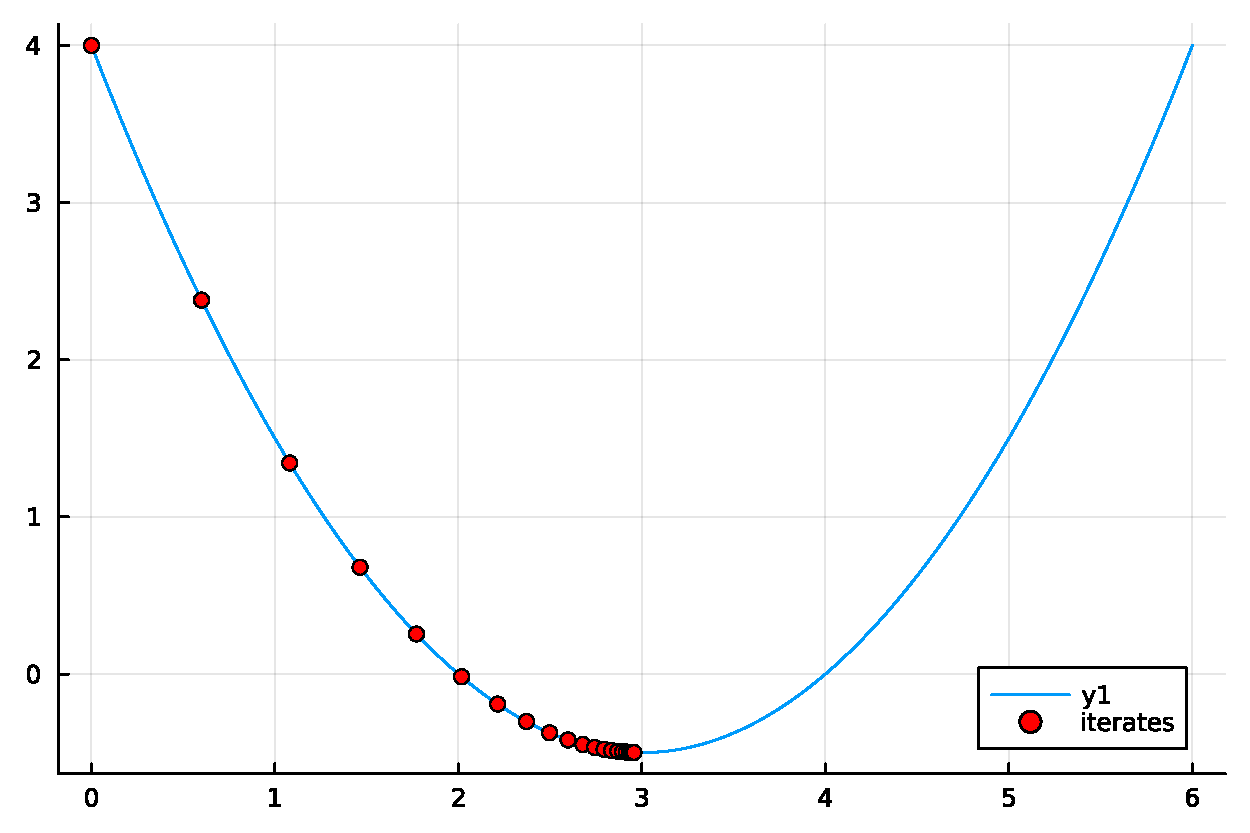
\includegraphics[width=.85 \linewidth]{crude1}
    \caption{$\alpha = 0.2$, iteration complexity = 20}
    \label{fig:crude1}
  \end{subfigure}%
  \begin{subfigure}{.5\textwidth}
    \centering
    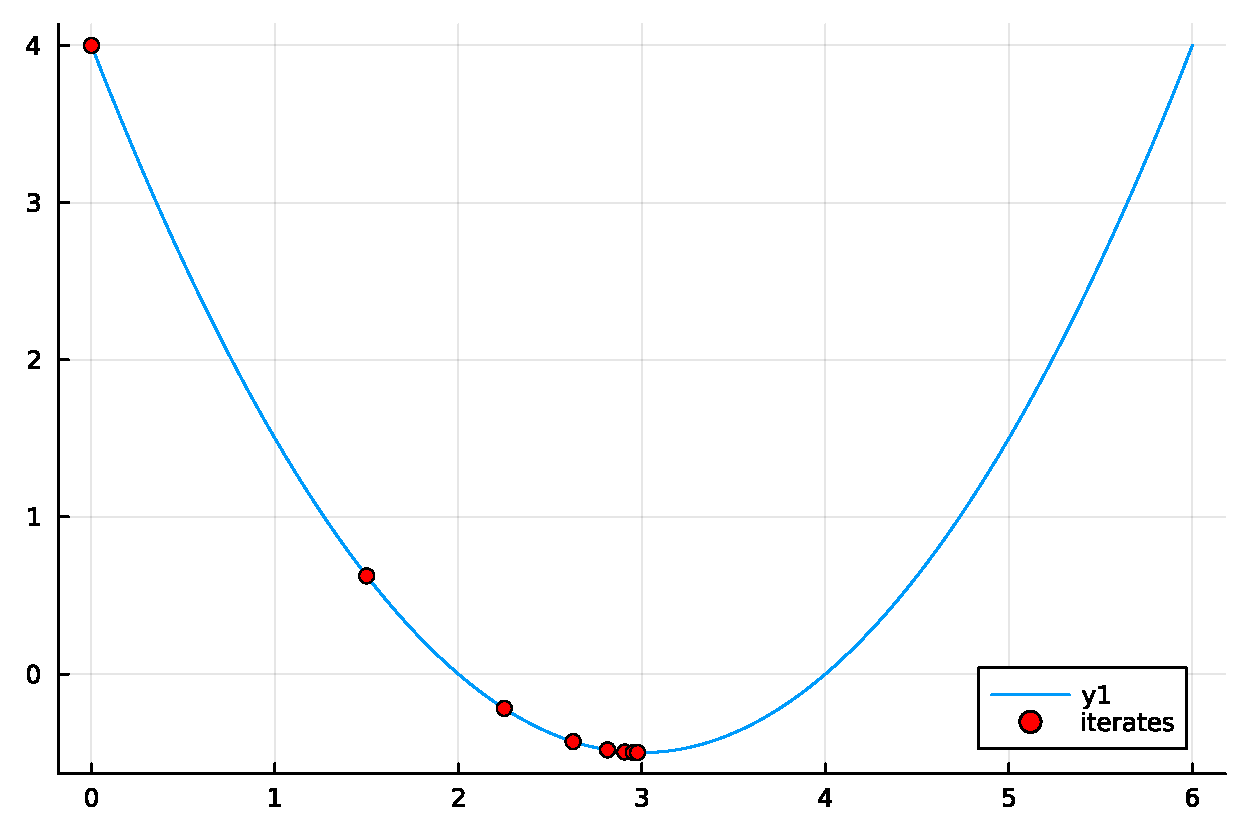
\includegraphics[width=.85 \linewidth]{crude2 }
    \caption{$\alpha = 0.5$, iteration complexity = 7}
    \label{fig:crude2}
  \end{subfigure}
  \begin{subfigure}{.5\textwidth}
    \centering
    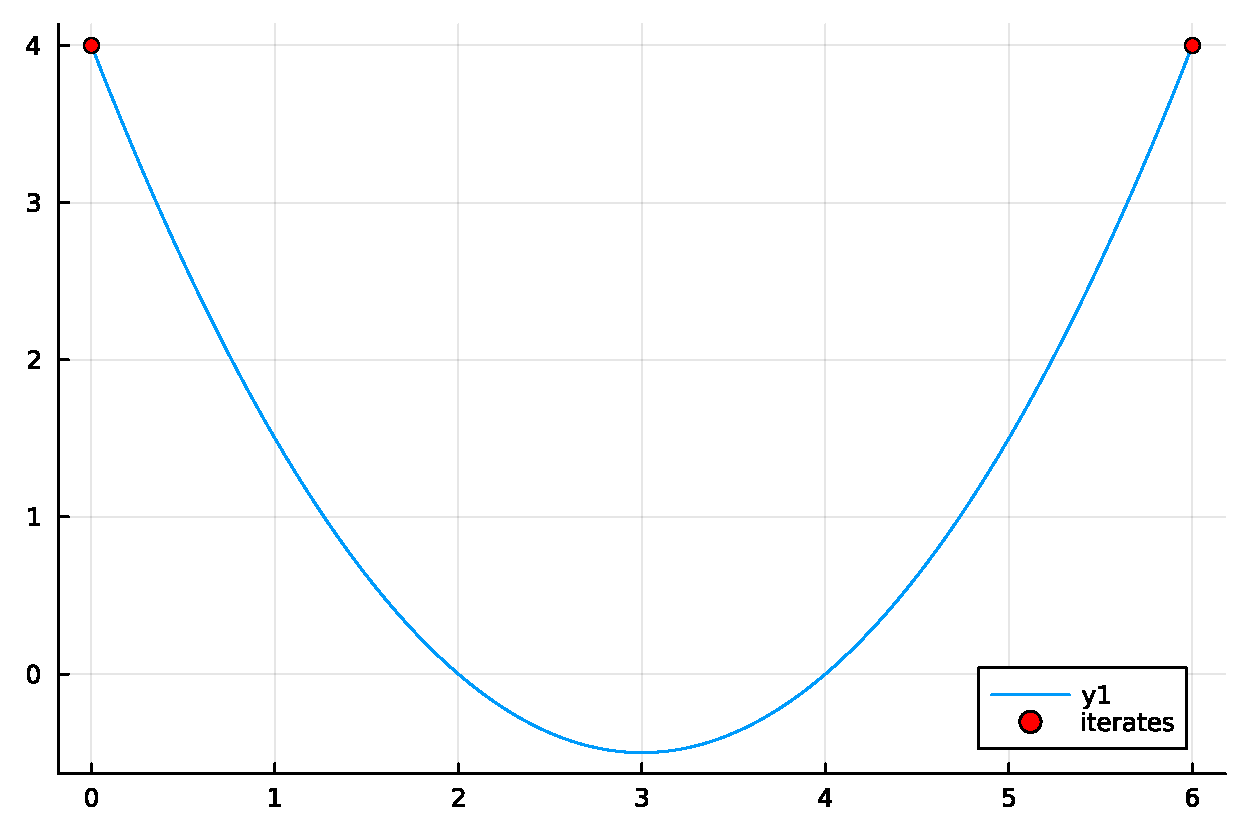
\includegraphics[width=.85 \linewidth]{crude3 }
    \caption{$\alpha = 2$, does not converge}
    \label{fig:crude3}
  \end{subfigure}
  \caption{Performance of 3 GD variants of different step sizes solving a quadratic function}
\label{fig:test}
\end{figure}

% \begin{figure}[htp]
%   \centering
%   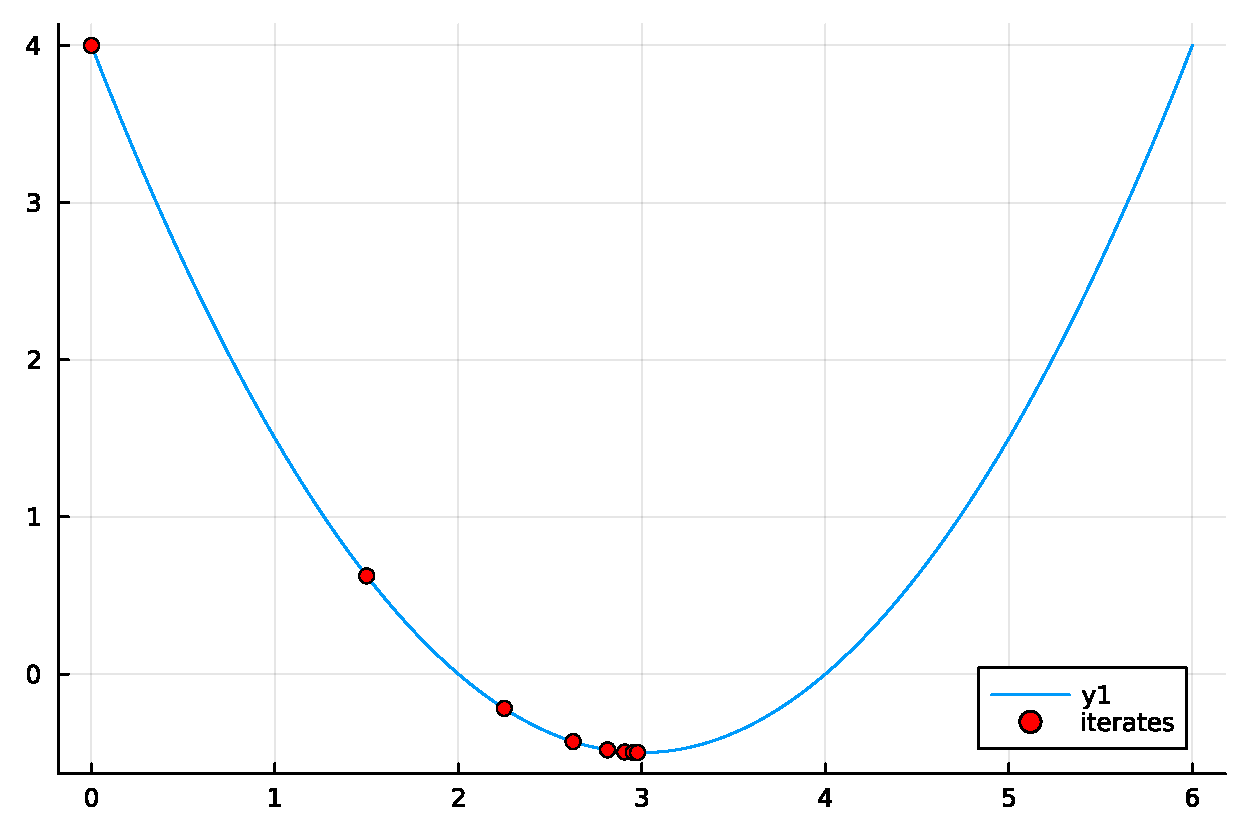
\includegraphics[width=.6\textwidth]{crude2}\hfill
%   \caption{$\alpha = 0.5$, iteration complexity = 21}
%   \label{fig:crude2}
% \end{figure}
% \begin{figure}[htp]
%   \centering
%   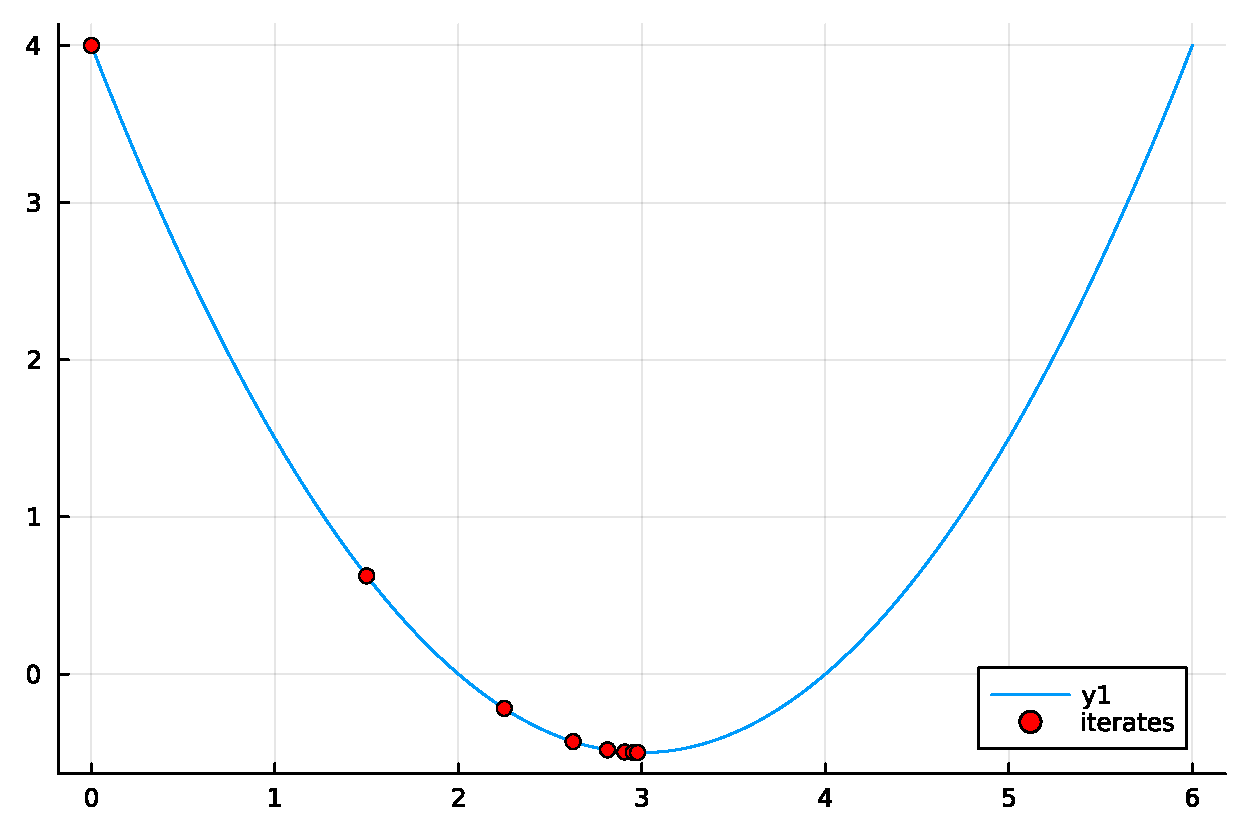
\includegraphics[width=.6\textwidth]{crude2}\hfill
%   \caption{$\alpha = 2$, does not converge}
%   \label{fig:crude3}
% \end{figure}

It can be seen how different tunings on the same algorithm can achieve drastically different speed optimizing a function, or whether it can solve for the minimum at all. Considering there exist many other first order methods in addition to the three in 1.1, each infinitely adjustable by changing the step size or by changing the number of past iterations used, being able to predict how an algorithm will perform can speed up the process of finding the best performing algorithm which can find a more accurate solution can be found and in fewer iterations. And while the example is of a simple function where overshoot can easily be identified and the number of iteration needed is small, the benefit of using an optimal algorithm only increases as the problem gets larger and more complex. In the application of training large language and self-driving models, the training process has taken place for many years and will continue as more training data is available and the models' continous improvement is desired. This training uses vast amounts of time and computational power, as a result, even a small improvement in the performance of the algorithm used can speed up the training process while reducing the energy needed.

Considering the quadratic function example, while it yielded an analysis of the algorithms' performance, it required solving the optimization problem. Not only would solving any problem large enough to warrant being optimized numerically in the first place computationally expensive, any benefit of finding a superior algorithm at solving a problem is negated as said problem has already been solved. Additionally, any analysis result is applicable only to one function and cannot be reliably used to derive a first-order method's performance on any other problem.

Due to these limitations, it is more efficient to analyze algorithms' performance at solving a broader set of problems. As a result of their widespread application, popular iterative gradient-based algorithms have been extensively analyzed. A frequently cited attempt is the Adam algorithm \cite{adam}, in which the performance of algorithms are compared using experiments and emperical evidence. There exists a different approach to quantifying the performance of algorithms, presented in \cite{drori2012}, \cite{taylor2016}, and \cite{lessard2016}, which aims to find a mathematically provable performance guarantee of an algorithm over a class of functions. This worst-case analysis is referred to as algorithm analysis: Given that a characteristic that a set of functions might share (such as being convex or quadratic), algorithm analysis would return the worst-case performance measure that guarantees the algorithm analyzed would perform as good or better at solving every function within said set.

\section{Julia programming language}

Algorithm Analysis is written in the Julia programming language, a high-level programming language designed specifically for high-performance numerical computing. Julia's compiler performance has been benchmarked to be faster than many other languages used for numerical computing while rivalling C, a language often used for its high efficiency \cite{julia}. Julia accomplishes this while being a high-level language with simple syntax rules that resembles existing popular languages, making it easy to develop and to understand.

Julia was also chosen as it is designed for numerical computing, supporting matrices as well as UTF-8 encoding, making it possible to use scientific notation: variables and functions as they exist in the code and as the user inputs them into the program can use math symbols or Greek letters. This makes Julia excel at communicating mathematical concepts, which simplifies both the process of coding the program and understanding its mathematical underpinnings.

Julia was also chosen as it is open-source and available for free. As Algorithm Analysis is a package designed for expert and novice users alike to install and use, it made sense to choose Julia as it is available on many of the popular platforms such as macOS, Windows, and Linux.

\section{Analysis Example}
To perform algorithm analysis with Algorithm Analysis, the user needs to follow the folliowing 3 steps:
\begin{enumerate}
	\item Choose from a supported list the class of function to be optimized.
	\item Define an algorithm to be analyzed .
	\item Specify a performance measure.
\end{enumerate}
In the Lyapunov-based method to analyzing algorithms and in Algorithm Analysis, a function class is defined as every functions which share a trait. In example \ref{ex_analysis}, the class of function is sector bounded between $m=1$ and $L=10$, which include any function $f$ that satisfy the condition:
\begin{equation}
  (\nabla f(x) - m(x-x_*))^\tp (\nabla f(x) - L(x-x_*)) \leq 0
\end{equation}
where $x_*$ is the global minimum of the function $f$
\begin{figure}[h!]
	\begin{lstlisting}[mathescape]
m,L = 1,10
$ \alpha $ = 2/(L+m)
@algorithm begin

	f = DifferentiableFunctional{R$ ^n $}()
	xs = first_order_stationary_point(f)
	f' $ \in $ SectorBounded(m, L, xs, f'(xs))

	x0 = R$ ^n $()
	x1 = x0 - $ \alpha $*f'(x0)

	x0 => x1

	performance = (x1-xs)^2
end

@show rate(performance)
\end{lstlisting}
\caption{Analysis Example}
\label{ex_analysis}
\end{figure} In the example code, the user:
\begin{itemize}
	\item Define the class of function \texttt{f} and its $\nabla f$, coded as \texttt(f') by calling one of the provided functions.
	\item Set the global minimum goal as a stationary point $ x_s $.
	\item Define an initial state $ x_0 $ and the algorithm with which its next state $ x_1$ is updated. In this example, the algorithm being analyzed is gradient descent with a step size $ \alpha = 2/11$.
	\item Set the performance measure as the norm distance between the initial state and the goal $ (x_0 - x_s)^2 $. The returned convergence rate guarantee is the rate at which the performance measure decreases after each iteration of the algorithm.
	\item Call the rate function to perform algorithm analysis.
\end{itemize}

With the calling of the rate function, Algorithm Analysis is ran automatically to return a rate of 0.6687164306640625. This is the converenge rate guarantee $\rho$ such that, for some performance measure $c>0$, it is upper bounded by $c \rho^k$ at each iteration $k$, for the provided algorithm and every function in the class. This guaranteed convergence rate using ``big-oh'' notation means that the performance measure converges with a minimum rate of $O(\rho^k)$. Throughout the process, the user never has to modify the package beyond providing its input or understand how Algorithm Analysis operate, making it an accessible tool.

\begin{figure}[hbtp]
  \begin{lstlisting}
  rate(performance) = 0.6687164306640625
  \end{lstlisting}
  \caption{Analysis result}
  \label{ex_result}
\end{figure}

\section{Overview} \label{sectionOverview}

% JuPE performs worst-case algorithm analysis when three main inputs are provided: the class of functions in question, the algorithm being analyzed, and a performance measure. The package then performs the algorithm analysis and returns the fastest guaranteed convergence rate.

% To use JuPE, an iterative first-order algorithm needs to be defined as an input to the program by specifying how it is updated. The class of function is provided by detailing the characteristic of the set, and a performance measure is defined. Throughout the process, the user never has to change the code of the package or understand how JuPE works, making it an easy to use black box tool.

%, such as 1 strong 10 smooth convex function, which can be how far the iterate \(x_k\) is from the goal \(x_*\) or any quadratic combinations of the iterates
Ater the introduction, in \Cref{chapter:literature}, the existing literature of approaches to analyzing algorithms and implementation into a program is presented. \Cref{chapter:lyapunov} discusses the Lyapunov-based mathematical method that Algorithm Analysis utilizes. In \Cref{chapter:code}, the main contribution of this thesis is presented: how a dommain-specific language is developed to support Algorithm Analysis's functionality. Finally in \Cref{chapter:result}, the analysis process and result are presented.

% \comment{Reference the specific chapters, such as Chapter~\ref{chapter:literature} (see the reference label at the beginning of that chapter for how to make the rerence).}